
% mnras_template.tex 
%
% LaTeX template for creating an MNRAS paper
%
% v3.0 released 14 May 2015
% (version numbers match those of mnras.cls)
%
% Copyright (C) Royal Astronomical Society 2015
% Authors:
% Keith T. Smith (Royal Astronomical Society)

% Change log
%
% v3.0 May 2015
%    Renamed to match the new package name
%    Version number matches mnras.cls
%    A few minor tweaks to wording
% v1.0 September 2013
%    Beta testing only - never publicly released
%    First version: a simple (ish) template for creating an MNRAS paper

%%%%%%%%%%%%%%%%%%%%%%%%%%%%%%%%%%%%%%%%%%%%%%%%%%
% Basic setup. Most papers should leave these options alone.
%\documentclass[fleqn,usenatbib]{mnras}
\documentclass[fleqn,usenatbib]{mnras}


% MNRAS is set in Times font. If you don't have this installed (most LaTeX
% installations will be fine) or prefer the old Computer Modern fonts, comment
% out the following line
%\usepackage{newtxtext,newtxmath}
% Depending on your LaTeX fonts installation, you might get better results with one of these:
%\usepackage{mathptmx}
%\usepackage{txfonts}

% Use vector fonts, so it zooms properly in on-screen viewing software
% Don't change these lines unless you know what you are doing
\usepackage{yfonts}
\usepackage[T1]{fontenc}
\usepackage{ae,aecompl}


%%%%% AUTHORS - PLACE YOUR OWN PACKAGES HERE %%%%%

% Only include extra packages if you really need them. Common packages are:
\usepackage{graphicx}	% Including figure files
\usepackage{amsmath}	% Advanced maths commands
\usepackage{amssymb}	% Extra maths symbols

\usepackage{hyperref}
%\usepackage{url}
%\usepackage{microtype}
%\usepackage{rotating}
\usepackage{booktabs}
\usepackage{threeparttable}
\usepackage{tabularx}
\usepackage{xspace}


%%%%%%%%%%%%%%%%%%%%%%%%%%%%%%%%%%%%%%%%%%%%%%%%%%

%%%%% AUTHORS - PLACE YOUR OWN COMMANDS HERE %%%%%

% Please keep new commands to a minimum, and use \newcommand not \def to avoid
% overwriting existing commands. Example:
%\newcommand{\pcm}{\,cm$^{-2}$}	% per cm-squared
\newcommand{\project}[1]{\textsl{#1}}
\newcommand{\nustar}{\project{NuSTAR}\xspace}
\newcommand{\fermi}{\project{Fermi}\xspace}
\newcommand{\rxte}{\project{RXTE}\xspace}
\newcommand{\xmm}{\project{XMM-Newton}\xspace}
\newcommand{\rosat}{\project{ROSAT}\xspace}
\newcommand{\swift}{\project{Swift}\xspace}
\newcommand{\astrosat}{\project{Astrosat}\xspace}
\newcommand{\ixpe}{\project{IXPE}\xspace}
\newcommand{\nicer}{\project{NICER}\xspace}

\newcommand{\given}{\ensuremath{\,|\,}}
\newcommand{\dd}{\ensuremath{\mathrm{d}}}
\newcommand{\counts}{\ensuremath{y}}
\newcommand{\pars}{\ensuremath{\theta}}
\newcommand{\mean}{\ensuremath{\lambda}}
\newcommand{\likelihood}{\ensuremath{{\mathcal L}}}
\newcommand{\Poisson}{\ensuremath{{\mathcal P}}}
\newcommand{\Uniform}{\ensuremath{{\mathcal U}}}

\newcommand{\Normal}{\ensuremath{{\mathcal N}}}
\newcommand{\bg}{\ensuremath{\mathrm{bg}}}
\newcommand{\word}{\ensuremath{\phi}}

%%%%%%%%%%%%%%%%%%%%%%%%%%%%%%%%%%%%%%%%%%%%%%%%%%

%%%%%%%%%%%%%%%%%%% TITLE PAGE %%%%%%%%%%%%%%%%%%%

% Title of the paper, and the short title which is used in the headers.
% Keep the title short and informative.
\title[]{The Likelihood for Cospectra in the Presence of Variability}

% The list of authors, and the short list which is used in the headers.
% If you need two or more lines of authors, add an extra line using \newauthor
\author[Huppenkothen et al.]{Daniela Huppenkothen$^{1}$ and Matteo Bachetti$^{2}$
\\
% List of institutions
   $^{1}$DIRAC Institute, Department of Astronomy, University of Washington, 3910 15th Avenue NE, Seattle, WA 98195, USA\\
   $^{2}$INAF-Osservatorio Astronomico di Cagliari, via della Scienza 5, I-09047 Selargius (CA), Italy \\
}


% These dates will be filled out by the publisher
\date{Accepted XXX. Received YYY; in original form ZZZ}

% Enter the current year, for the copyright statements etc.
\pubyear{2017}

% Don't change these lines
\begin{document}
\label{firstpage}
\pagerange{\pageref{firstpage}--\pageref{lastpage}}
\maketitle

% Abstract of the paper
\begin{abstract}
Likelihoods for cospectra are hard!
\end{abstract}

% Select between one and six entries from the list of approved keywords.
% Don't make up new ones.
\begin{keywords}
X-rays:binaries -- X-rays:individual -- stars:black holes -- methods:data analysis -- methods:statistical
\end{keywords}

\section{Introduction}

Cospectra for white noise were straightforward, but we kind of want to fit cospectra with parametric models, too, so we need a likelihood. This is much harder, as we'll show below.

\section{Cospectra of Stationary Random Processes}

For most stationary random processes (e.g.\ red noise or quasi-periodic oscillations, QPOs), the power spectrum is conveniently distributed as $\chi^2_2$ around the underlying power spectral process $P(\nu)$ that generated the data. This is not true for co-spectra, but neither can the equations defined in \citet{huppenkothen2018} be used. The reason lies in the fact that the Fourier amplitudes $A_{xj}$ and $A_{yj}$ are no longer statistically independent from each other (and neither are $B_{xj}$ and $B_{yj}$). In this section, we show that the general likelihood for correlated light curves has no closed form unless the correlation is exactly $1$, in which case the algorithm recovers the exact $\chi^2_2$ distribution expected for power spectra, or $0$, which reproduces the statistical distributions for white noise cospectra in \citet{huppenkothen2018}. %Periodicity detection can be performed in the white noise regime via the probabilities derived in Sections \ref{sec:detection_thresholds} and \ref{sec:averaged_cospectra} above. For candidate frequencies within a part of Fourier space dominated by a non-white stochastic process, one must first estimate the underlying spectral density, and then simulate from this process in order to calibrate the false-alarm probability.

\subsection{The Cospectrum}

Consider two stationary, evenly-sampled time series $\mathbf{x} = \{x_k\}_{k=1}^N$ and $\mathbf{y} = \{y_k\}_{k=1}^N$ with no gaps. Further assume that these time series were recorded with identical detectors and differ only in the noise introduced by the measurement process (e.g.\ photon counting statistics), while the underlying source variability is identical for both time series. The simplest possible case---that of pure white noise---was examined in \citet{huppenkothen2018}. In the following, we will consider the case of a stationary random process (such as a red noise process or a quasi-periodic oscillation) shared between $\mathbf{x}$ and $\mathbf{y}$, with each time series independently affected by some white noise process (e.g.\ Gaussian noise). 

In this case, we have for some data point $x_k = s_k + n_{xk}$ and $x_k = s_k + n_{yk}$, where $n_{xk}$ and $n_{yk}$ are drawn independently from the same distribution, and $s_k$ is a stationary random process shared between the two light curves. Define the Fourier transform of each time series as

\begin{eqnarray}
\mathcal{F}_x(j) &=& \frac{1}{2}(A_{xj} - i B_{xj}) \exp{-i\left(\frac{2\pi j t}{T}\right)} \\
\mathcal{F}_y(j) &=& \frac{1}{2}(A_{yj} - i B_{yj}) \exp{-i\left(\frac{2\pi j t}{T}\right)}
\end{eqnarray}

\noindent where $i = \sqrt{-1}$, and $A_{xj}$, $A_{yj}$, describe the real components, $B_{xj}$, $B_{yj}$ the imaginary components of the Fourier amplitudes at a given frequency $\nu_j$, respectively. We restrict $\nu_j$ to lie between $\nu_0 = \frac{1}{T}$, where $T$ is the total length of the time series, and the Nyquist frequency, $\nu_{j=N/2} = 1/(2\Delta t)$ for a time resolution $\Delta t$. 
he complex cross spectrum for the time series $\mathbf{x}$ and $\mathbf{y}$ is given by

\begin{eqnarray}
\label{eqn:crossspectrum}
\mathcal{F}_x(j) \mathcal{F}_y^*(j) & = & \frac{1}{2} (A_{xj} - i B_{xj}) e^{i \frac{2 \pi j t}{T}} \frac{1}{2} (A_{yj} + i B_{yj}) e^{i \frac{-2 \pi j t}{T}}\nonumber \\ 
		     & = & \frac{1}{4} [ (A_{xj}A_{yj} + B_{xj}B_{yj}) + \\\nonumber
		     & &  i (A_{xj}B_{yj} - A_{yj}B_{xj}) ]
\end{eqnarray}


\noindent For the combination of stochastic processes assumed here,  we can use the Poisson summation formula to write the Fourier amplitudes as a sum of the contributions from the signal and the noise component:

\begin{eqnarray}
A_{xj} &=& A_{xsj} + A_{xnj} \nonumber \\
B_{xj} &=& B_{xsj} + B_{xnj} \, ,
\end{eqnarray}

\noindent where $A_{xsj}$ and $B_{xsj}$ denote the real and imaginary components of the signal power in the Fourier amplitudes at frequency $\nu_j$ derived from the light curve $\mathbf{x}$, and $A_{xnj}$ and $B_{xnj}$ similarly denote the white noise components in the Fourier amplitudes at the same frequency (identical expressions hold for $\mathbf{y}$). 

For a large enough number of data points $N$, the Fourier amplitudes $A_{xj}$ and $B_{xj}$ will be composed of a sum of two independent random normal variables, with $A_{xsj} \sim \Normal(0, \sigma^2_{sj})$ and $A_{xnj} \sim \Normal(0, \sigma^2_n)$, where the signal variance

\begin{equation}
\label{eqn:variance}
\sigma^2_{sj} = \sigma^2_{s}(\nu_j) = N_\mathrm{phot} \frac{P_j}{4}
\end{equation}

\noindent is given by the power spectrum of the underlying stochastic process, $P_j = P(\nu_j)$, and $N_{\mathrm{phot}} = \sum_{k=1}^{N}{x_k}$ is the integrated flux in the light curve. We also have $\sigma^2_n = N_\mathrm{phot}/2$, and hence the combined distributions become

\begin{eqnarray}
A_{xj} \sim \Normal(0, \sigma^2_{sj}+\sigma^2_{n}) \nonumber \\
A_{yj} \sim \Normal(0, \sigma^2_{sj}+\sigma^2_{n}) \, . \nonumber
\end{eqnarray}

\noindent Similar expressions can be found for $B_{xj}$ and $B_{yj}$, respectively. It is important to note that $A_{xsj} = A_{ysj}$ and similarly $B_{xsj} = B_{ysj}$, that is, the amplitudes of the stationary noise process will be the same for the Fourier transforms of $\mathbf{x}$ and $\mathbf{y}$, while the components due to white noise \textbf{differ} between the two time series, since the latter is due to measurement noise in the two independent detectors. This has important consequences for the sampling distribution of the cospectrum. Most importantly, as we will see below, the \textit{statistical distribution} of each cospectral power $C_j$ will itself be a function of frequency,  because it directly depends on the amplitude of the variance supplied by the stationary stochastic process versus the white noise contribution.

\subsubsection{Correlation Coefficient}

It is instructive and useful to derive the Pearson product moment correlation coefficient [REF] for the two Fourier amplitudes given the assumptions above.
The correlation between Fourier amplitudes $A_{xj}$ and $A_{yj}$ (and similarly between the other components) depends directly on the fraction of variance shared between the two light curves: the central normal distribution that all components adhere to implies $E[A_{xj}] = E[A_{yj}] = E[B_{xj}] = E[B_{yj}] = 0$, whereas the expectation of the product is set by the underlying stochastic process $E[A_{xj}A_{yj}] = E[B_{xj}B_{yj}] = (\sigma_{sj}^2)^2$. 
We thus have for the covariance 

\[
\mathrm{cov}(A_{xj}, A_{yj}) = \sigma_{sj}^2 \; ,
\]

\noindent and furthermore for the correlation coefficient

\begin{equation}
r_j = \frac{\mathrm{cov}(A_{xj}, A_{yj})}{\sqrt{\sigma_{A_{xj}}^2\sigma_{A_{yj}}^2}} = \frac{\sigma_{sj}^2}{ (\sigma_{sj}^2 + \sigma_{n}^2)} \; ,
\end{equation}

\noindent which for the assumption of a shared stationary stochastic process and independent white noise becomes

\begin{equation}
r_j = \frac{N_{\mathrm{phot}}P_j/4}{\left(\frac{N_{\mathrm{phot}}}{4}P_j + \frac{N_{\mathrm{phot}}}{2}\right)} = \frac{P_j}{P_j + 2}\; .
\label{eqn:corrcoeff}
\end{equation}

\subsubsection{The Product of Correlated Gaussian Random Variables}

According to Equation \ref{eqn:crossspectrum}, the cospectrum, defined as the real part of the cross spectrum, is defined as 

\begin{equation}
\label{eqn:cospectrum}
C_j = \frac{1}{2}(A_{xj} A_{yj} + B_{xj} B_{yj} 
\end{equation}

\noindent at a given frequency $\nu_j$. All four terms in this equation are random variables drawn from the same normal distribution with zero mean and variance $\sigma**2 = \sigma_{sj} + \sigma_n$, and are correlated among each other with correlation coefficient $r_j$ as defined in Equation \ref{eqn:corrcoeff}. Thus, the cospectral power $C_j$ is the sum of two products of these normally distributed random variables.

%Deriving the sampling distribution of the cospectral powers $C_j = (A_{xj}A_{yj} + B_{xj}B_{yj})$ requires summation of two random variables following the probability density function (PDF) defined in Equation \ref{eqn:varsquaredamp}. In practice, this requires the convolution of the PDFs of the two random variables to be added. Because this convolution is difficult to calculate directly, it is instructive to consider the \textit{moment-generating function} of the PDF instead, defined as

\citet{craig1936} first derived the moment-generating function for the product of two normally distributed random variables with arbitrary means, variances and correlation coefficients. In general, the moment-generating function of a statistical distribution is defined as

\begin{equation}
M_Z(t) := \mathbb{E}[e^{tZ}] \, 
\end{equation}

\noindent for a random variable $Z$. For the product of Gaussian random variables, this equation becomes

\begin{equation}
M_{A_{xj}A_{yj}}(t) = \frac{\exp{\left( \frac{(\rho_x^2 + \rho_y^2 - 2r\rho_x \rho_y)t^2 + 2 \rho_x\rho_y t}{2[1 - (1 + r)t][1 + (1-r)t]}\right)}}{\sqrt{[1-(1+r)t][1+(1-r)t]}} \; ,
\end{equation}

\noindent where $\rho_x = \mu_{A_{xj}}/\sigma_{A_{xj}}$ and $\rho_y = \mu_{A_{yj}}/\sigma_{A_{yj}}$. The probability density function corresponding to this moment-generating function was derived for the most general case in terms of an infinite sum of modified Bessel functions by \citet{cui2016}, who also studied the approximation error and the convergence rate when finite summations are exploited. 

In the case presented here, $\rho_x = \rho_y = 0$ because the means for both amplitude components are zero. In this case, the distribution simplifies to 

\begin{equation}
M_{A_{xj}A_{yj}}(t) = \frac{1}{\sqrt{[1-(1+r)t][1+(1-r)t]}} \, .
\label{eqn:varmgf}
\end{equation}

\noindent Note once again that the moment-generating function depends on the correlation coefficient $r$, and thus if $r$ is a function of frequency $r = r(\nu)$, the \textit{sampling distribution} for the cospectral powers will also depend on frequency. 

The sums of two \textit{independent} variables with a probability distribution given in Equation \ref{eqn:varsquaredamp} can be described as the multiplication of their moment generating function. In the case of white noise only, the two terms in the sum in Equation \ref{eqn:cospectrum} are independent, thus the moment-generating function reduces to 

\begin{equation}
M_{C_j}(t) = \frac{1}{[1-(1+r)t][1+(1-r)t]} \, .
\label{eqn:varmgf2}
\end{equation} 

\noindent There are two special cases of interest. In particular, for independent random variables $r=0$, and hence the equation above reduces to 

\[
M_{C_j}(t) = \frac{1}{1-t^2} \, .
\]

\noindent This is the moment generating function of a Laplace distribution, derived for the white noise case in \citet{huppenkothen2018}. Conversely, for $r=1$, the Fourier amplitudes are exactly equal, $A_{xj} = A_{yj}$ and $B_{xj} = B_{yj}$,, and the above equation reduces to

\[
M_{C_j}(t) = \frac{1}{1-2t} \, ,
\]

which in turn is the moment generating function of a $\chi^2_2$ distribution, and we have recovered the distribution expected for power spectral densities.

In the general case of a stochastic process present in the time series, $r \neq 0$. For this special case, \citet{nadarajah2016} have shown that the probability density of the product of two Gaussian random variables with zero means, and arbitrary variances $\sigma_x^2$ and $\sigma_y^2$, and correlation coefficient $r$ can be written as

\begin{eqnarray}
f_{A_{xj}A_{yj}}(x) & = & \frac{1}{\sigma_{A_{xj}}\sigma_{A_{yj}} \sqrt{1 - r^2}} \exp{\left( \frac{rx}{\sigma_{A_{xj}}\sigma_{A_{yj}}(1-r^2)} \right)} \nonumber \\
 & & \times K_0\left( \frac{|x|}{\sigma_{A_{xj}}\sigma{A_{yj}}(1-r^2)} \right) \; ,
\label{eqn:varsquaredamp}
\end{eqnarray}

\noindent where $K_0$ is the Bessel function of the second kind of order $0$. Comparing to Equation [REF] in \citet{huppenkothen2018}, the PDF depends on the correlation coefficient $r$ and that compared to the simple case of white noise only, another exponential term was introduced. For $r=0$, the equation above reduces to the white noise case in \citet{huppenkothen2018}), as expected. \citet{nadarajah2016} also proved the probability density of the geometric mean of $K$ independent and identically distributed random variables drawn from Equation \ref{eqn:varsquaredamp}, and \citet{gaunt2018} showed that both Equation \ref{eqn:varsquaredamp} and the geometric mean are particular cases of a \textit{variance-gamma distribution}. The geometric mean $\bar{Z} =  \frac{1}{K} (Z_1 + Z_2 + ... + Z_n$ of $n$ variables, each a product $Z = XY$ is defined as

\begin{eqnarray}
\label{eqn:idp_pdf}
p_{\bar{Z}}(z) & = & \frac{n^{(n+1)/2} 2^{(1-n)/2} |z|^{(n-1)/2}}{(\sigma_x \sigma_y)^{(n+1)/2} \sqrt{\pi (1 - r^2)} \Gamma(n/2)} \\ \nonumber
       & & \times \exp{\left( \frac{r n z}{\sigma_x \sigma_y (1-r^2)} \right)} K_{\frac{n-1}{2}}\left( \frac{n |z|}{\sigma_x \sigma_y (1 - r^2)}  \right) \; ,
\end{eqnarray}

\noindent where $K_\tau$ is the Bessel function of the second kind of order $\tau$. If the real and imaginary components of the Fourier amplitudes were statistically independent, then Equation \ref{eqn:idp_pdf} with $n=2$ would provide the exact sampling distribution for the cospectrum. However, because $A_{xj}$ and $B_{xj}$ are correlated, the PDF above will, at best, be an approximation, and the more general case of all four Fourier amplitude components being correlated is likely to either have no or a very complicated closed-form solution (Gaunt, private communication).


\begin{figure*}
\begin{center}
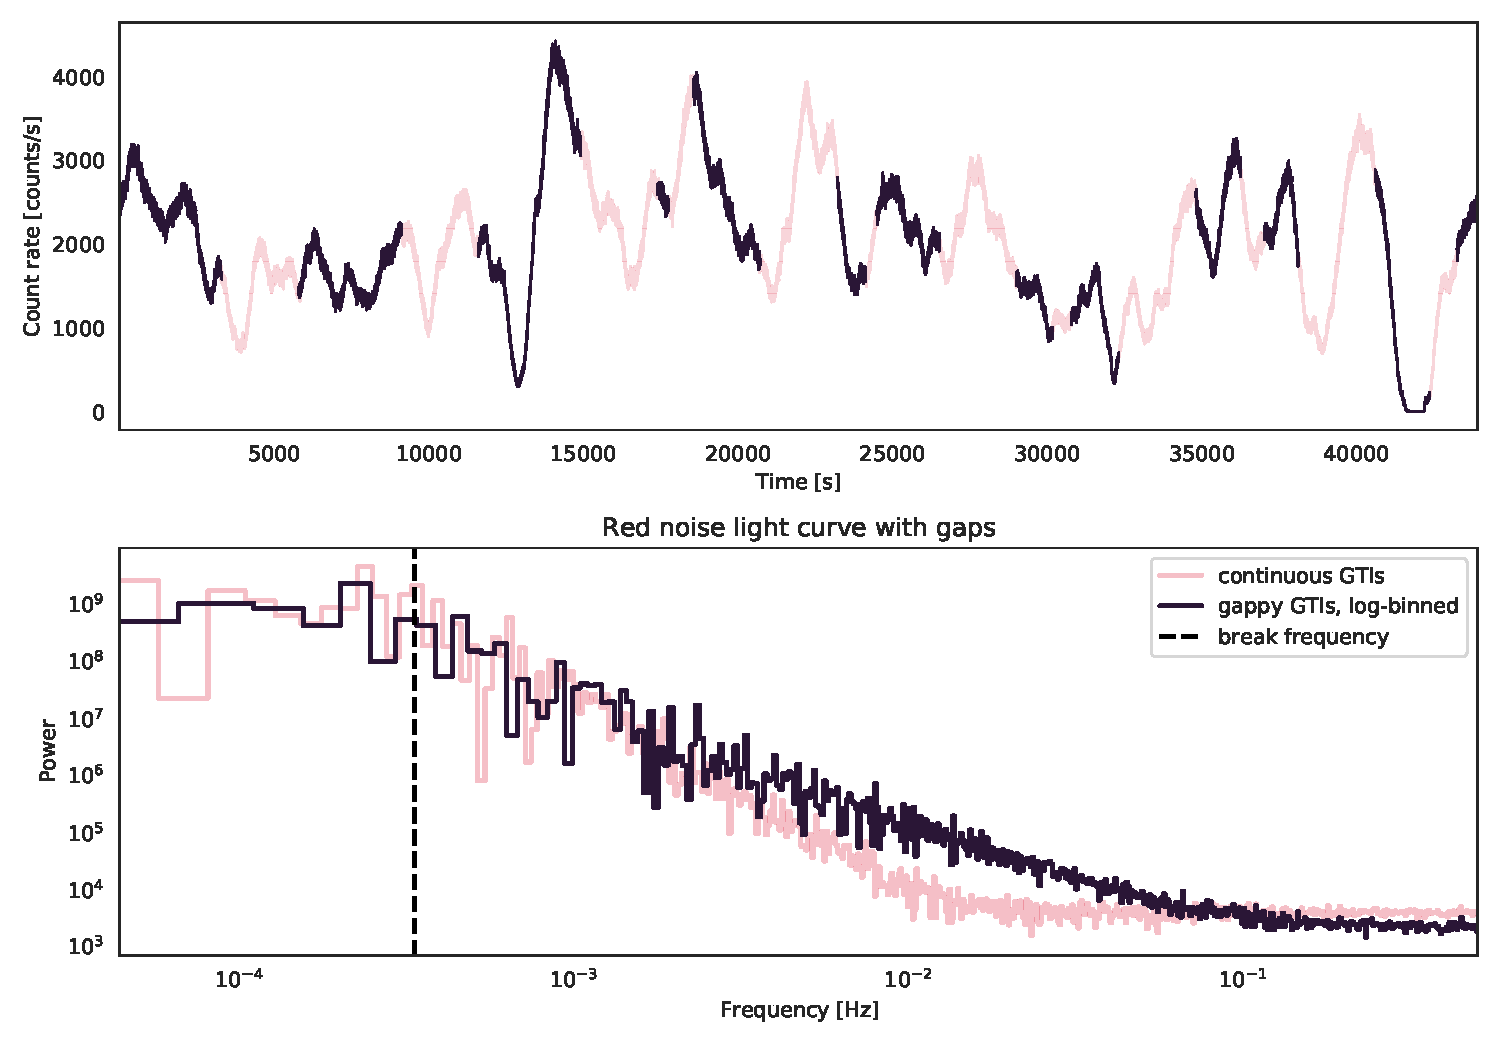
\includegraphics[width=\textwidth]{../figs/rednoise_psd.pdf}
\caption{Power spectral densities from averaging together one realization from all simulated data sets (left, black) with the model power spectrum (left, red) overplotted. In the right panel, we show the correlation coefficients in each frequency bin as a function of frequency $\nu$. As expected the red noise process causes the real part of the Fourier amplitudes to be strongly dominated at low frequencies, where the red noise contribution is strongest. The correlation drops sharply as the red noise weakens, and is nearly zero at high frequencies where white noise dominates.}
\label{fig:rednoise_psd}
\end{center}
\end{figure*}

\begin{figure*}
\begin{center}
\includegraphics[width=\textwidth]{../figs/rednoise_bessel.pdf}
\caption{Distribution of $A_{xj}A_{yj}$, the real parts of the Fourier amplitudes of the simulated light curves, for a large sample of $5000$ simulated light curves. We picked distributions for three different frequencies in cospectrum, and thus show the dependence of the sampling distribution for each frequency $\nu$ with frequency (via the dependence of the correlation coefficient $r_j = r(\nu_j)$ on \ frequency).  In grey, we show a fine-grained histogram of simulated amplitudes derived from $5000$ simulations. In red, we add the theoretical expected distribution from Equation \ref{eqn:varsquaredamp}. At low frequencies, where $r \approx 1$, the distribution is heavily skewed towards positive values, similar to what is expected from a $\chi^2$ distribution (left panel). As $r$ drops as a function of frequency with the power supplied by the stochastic process, the distribution becomes more and more symmetric (middle panel), until it approximates the symmetric Laplace distribution expected for uncorrelated noise (right panel).}
\label{fig:rednoise_bessel}
\end{center}
\end{figure*}

\subsubsection{Simulations}
\label{sec:rednoisesims}

We simulated light curves with $1000$ data points and a total duration of $10\,\mathrm{s}$ from a red noise process with a power spectrum distributed as a power law, $P(\nu) = A\nu^{-\alpha}$ with $\alpha=-2$. We used the well-known algorithm by \citet{timmer1995} to simulate light curves with a mean count rate of $10^{6}\,\mathrm{counts}/\mathrm{s}$ and a fractional rms amplitude of the red noise process, $f_\mathrm{rms} = 0.2$. We simulated the observations seen e.g.\ in two separate detectors in the same instrument by sampling from a Poisson distribution twice for each time bin with a rate equal to the flux in that bin given by red noise process. This yields two light curves that share the underlying stochastic process, but are different realizations of the same white noise process.

We then computed cospectral powers from the two light curves, and repeated the entire process $20,000$ times in order to build enough simulated data sets to explore their statistical properties. In Figure \ref{fig:rednoise_psd} we show the power spectrum (for illustration, rather than the co-spectrum) averaged over all simulations, using one of the two realizations. In order to probe the correlation between Fourier amplitudes, we used the set of real Fourier amplitudes in a given frequency bin $\nu$ for each realization and computed the correlation coefficient with the set of real Fourier amplitudes from the set of second realizations. As expected, we see a strong correlation between the real part of the Fourier amplitudes at low frequencies, where the red noise component dominates heavily over the white noise. Conversely, as the red noise becomes weaker with higher frequency, the correlation drops to nearly zero for the highest frequencies. The simulated correlation coefficients match exactly with the theoretical prediction in Equation \ref{eqn:corrcoeff}.

In Figure \ref{fig:rednoise_bessel}, we show distributions empirically derived from the simulated light curves for $A_{xj}A_{yj}$, for which an analytical expression exists. We pick three frequencies to give a representative overview of how the distribution of $A_{xj}A_{yj}$ depends on frequency. At low frequencies, the correlation between $A_{xj}$ and $A_{yj}$ is strong, as expected, because the power spectrum is dominated by the power supplied by the stochastic process. The resulting distribution is heavily skewed. As the red noise power drops as a function of frequency, the sampling distribution of $A_{xj}A_{yj}$ becomes increasingly less skewed, and approximates the expected Laplace distribution at high frequencies, where $r \approx 0$. The empirically derived correlation coefficient follows the theoretical expectation given in Equation \ref{eqn:corrcoeff}.


\begin{figure}
\begin{center}
\includegraphics[width=0.5\textwidth]{../figs/pl_tvs.pdf}
\caption{Estimating the distance between the empirical distribution of cospectra derived from simulations of red noise light curves, and the probability density defined in Equation \ref{eqn:idp_pdf}. We measure the Total Variation Distance as defined in Equation \ref{eqn:tvs} at each frequency $\nu_j$. In the top panel, we show one realization of the underlying power spectrum: the light curves were simulated from a power-law power spectrum with a power spectral index of $\Gamma = 2$, using \citet{timmer1995}, and then Fourier-transformed to show the realization depicted here. Middle panel: the Total Variation Distance as a function of frequency bin $j$ (black), along with the mean (red dashed) and the $95^{\mathrm{th}}$ (teal dot-dashed) percentile of the baseline distribution for the TVD derived from random draws of correlated bivariate normal random variables. The TVD at low frequencies is significantly higher than the baseline distribution, indicating that there is a mismatch between the empirical distribution cospectral powers and the PDF. At high frequencies, white noise dominates the spectrum, and since in this regime the Fourier amplitudes are largely uncorrelated, the distance between the PDF in Equation \ref{eqn:idp_pdf} and the distribution of cospectra is similar to that found from the reference distribution. The same behaviour is mirrored in the bottom panel, which shows as a function of frequency the $p$-value of observing the distribution of cospectra under the assumption that the PDF is a good model. This null hypothesis can be rejected for small frequencies, where the red noise dominates and the $p$-value is very small (zero in most cases here, due to the finite number of simulations in the reference distribution). At high frequencies in the white noise-dominated regime, the $p$-value is essentially randomly drawn from a uniform distribution, indicating that the null hypothesis cannot be rejected.}
\label{fig:tvs}
\end{center}
\end{figure}


\begin{figure}
\begin{center}
\includegraphics[width=0.5\textwidth]{../figs/plqpo_tvs.pdf}
\caption{Estimating the distance between the empirical distribution of cospectra derived from simulations of red noise light curves, and the probability density defined in Equation \ref{eqn:idp_pdf}. We measure the Total Variation Distance as defined in Equation \ref{eqn:tvs} at each frequency $\nu_j$. In the top panel, we show one realization of the underlying power spectrum: the light curves were simulated from a power-law power spectrum with a power spectral index of $\Gamma = 2$, using \citet{timmer1995}, and then Fourier-transformed to show the realization depicted here. Middle panel: the Total Variation Distance as a function of frequency bin $j$ (black), along with the mean (red dashed) and the $95^{\mathrm{th}}$ (teal dot-dashed) percentile of the baseline distribution for the TVD derived from random draws of correlated bivariate normal random variables. The TVD at low frequencies is significantly higher than the baseline distribution, indicating that there is a mismatch between the empirical distribution cospectral powers and the PDF. At high frequencies, white noise dominates the spectrum, and since in this regime the Fourier amplitudes are largely uncorrelated, the distance between the PDF in Equation \ref{eqn:idp_pdf} and the distribution of cospectra is similar to that found from the reference distribution. The same behaviour is mirrored in the bottom panel, which shows as a function of frequency the $p$-value of observing the distribution of cospectra under the assumption that the PDF is a good model. This null hypothesis can be rejected for small frequencies, where the red noise dominates and the $p$-value is very small (zero in most cases here, due to the finite number of simulations in the reference distribution). At high frequencies in the white noise-dominated regime, the $p$-value is essentially randomly drawn from a uniform distribution, indicating that the null hypothesis cannot be rejected.}
\label{fig:plqpo_tvs}
\end{center}
\end{figure}

\subsubsection{Measuring the Distance Between The True and Empirical Distribution}

In order to better understand how close the approximation is to the true distribution, we used the simulations above to build an empirical density for the cospectral power $C_j$ at each frequency $\nu_j$, and compared this distribution to the pdf defined in Equation \ref{eqn:idp_pdf} with $n=2$. In order to generate a baseline distribution, we simulated random variables from a bivariate normal distribution with zero means, the equal variance of $\sigma_x = \sigma_y = 4.22$ and a covariance of $0.88$. We simulated $40,000$ pairs of random variables in this way, the computed the product of these pairs. In order to approximate the cospectrum, we then took the first half of this vector, and added the second half of the vector to the first, generating a total of $20,000$ random variables constructed out of the sum of two variables, each of which is the product of a pair of correlated zero-mean Gaussian draws. This distribution should follow equation \ref{eqn:idp_pdf} exactly [ADD PLOT]. In order to understand how well Equation \ref{eqn:idp_pdf} matches the cospectral powers, we calculate the Total Variation Distance, defined as 

\begin{equation}
\label{eqn:tvs}
||X - Y||_\mathrm{tv} = \frac{1}{2} \sum_{x \in \Omega}|\mu(x) - \eta(x)| \; ,
\end{equation}

\noindent, which describes the largest difference in probability, taken over all possible events, as the area between the two curves, $\mu(x)$ and $\eta(x)$. In practice, we compute a histogram with $200$ bins using the $20,000$ random samples above, and compare the normalized histogram to the integrated probability expected from Equation \ref{eqn:idp_pdf} in the same bin. We note that the histogram binning introduces a factor of uncertainty into our results, but repeated experiments with different binning factors yield only minor quantitative differences that do not affect our conclusions.

We repeat the above procedure $30,000$ times, calculating the total variation distance (TVD) each time for a sample of $20,000$ random numbers. This distribution serves as a baseline for the total variation distances we would expect under the assumption that our sample is randomly drawn from the probability distribution in Equation \ref{eqn:idp_pdf}. We then use the simulations generated in Section \ref{sec:rednoisesims} to construct distributions of $20,000$ cospectral powers $C_j$ for each frequency $\nu_j$. For each distribution, we calculate the total variation distance between the histogram of cospectral powers and the expected theoretical distribution under the (incorrect) assumption that the pairs of products of random normal variables are uncorrelated. 

In Figure \ref{fig:tvs}, we show an example realization of the power law power spectrum (top panel), and the total variation distance for each frequency $\nu_j$. We find that the total variation distance between the cospectral powers and the expected theoretical distribution depends strongly on frequency, and that this distance is systematically larger for smaller frequencies, indicating a systematic deviation from the expected distribution in the part of the cospectrum where the red noise dominates. For the highest frequencies, i.e.~ the white noise-dominated part of the cospectrum, the total variation distance follows the same distribution as when we generated random normal variables from the correct distribution. This is expected, since in this part of the cospectrum, the Fourier amplitudes are largely uncorrelated, and thus Equation \ref{eqn:idp_pdf} should be a reasonable approximation. Where red noise dominates, however, the TVD grows, and Equation \ref{eqn:idp_pdf} may not be an appropriate approximation. This can also be observed in the bottom panel of Figure \ref{fig:tvs}, where we show the $p$-value derived from the empirical distribution for the TVD under the assumption that Equation \ref{eqn:idp_pdf} is correct, again as a function of frequency. At low frequencies, the $p$-value is systematically small, at the level of a few percent or less. For draws from the null hypothesis, we would expect the $p$-value to be uniformly distributed between $0$ and $1$, which is observed at higher frequencies, where white noise dominates. While for most frequencies, the $p$-value is not small enough to firmly reject the null hypothesis, the systematic trend to smaller $p$-values indicates that there is a process that is not entirely modelled by the null distribution.

In order to be able to make that statement more broadly, we also simulated light curves from a power spectrum that includes both a power law red noise component at low frequencies, as well as a strong quasi-periodic oscillation (QPO) superimposed on the red noise component. We simulate $20,000$ light curve realizations from this power spectrum as well, and compute the cospectrum for each, then repeat the procedure above and compute the total variation distance for each frequency $\nu_j$. In Figure \ref{fig:plqpo_tvs}, we present the cospectrum of  a realization of the stochastic process, the total variation distance as a function of frequency, and the $p$-value of that distance at a given frequency compared to a reference distribution drawn from the PDF in Equation \ref{eqn:idp_pdf}. As with the light curves simulated from only a power law, we find that the total variation distance is systematically larger at lower frequencies, and we find that the signal of the QPO can be traced in the total variation distance as well. This is expected: at the frequencies where the QPO is strongest in the cospectrum, the correlation between Fourier amplitudes will be highest, and thus the deviations from Equation \ref{eqn:idp_pdf} largest. As for the power law case, the $p$-value systematically trends to small values at low frequencies, though for any given frequency, it never becomes small enough to reject the null hypothesis at the $3\sigma$ level. 


\begin{figure}
\begin{center}
\includegraphics[width=0.5\textwidth]{../figs/test_pl_nodeadtime_alpha_0_fit.pdf}
\caption{}
\label{fig:plfit}
\end{center}
\end{figure}



\subsection{The Correlation Introduced by Variability matters}

While the total variation distance is a useful measure to quantify how close the empirical distribution of cospectral powers matches the PDF, it tells us little about what effect the distance between the two distribution makes in practice. In order to quantify this effect, we constructed a likelihood as

\begin{equation}
\label{eqn:likelihood}
\mathcal{L}(\theta) = \prod_{j=1}^{N/2}p(C_j | P_j) \; ,
\end{equation}

\noindent where $P_j = P(\nu_j, \theta$, is a power spectral model that is a function of frequency and parameters $\theta$, and $p(C_j | P_j)$ is defined in Equation \ref{eqn:idp_pdf}. $\sigma_x$, $\sigma_y$, and $r$ are calculated from $P_j$ using Equations \ref{eqn:variance} and \ref{eqn:corrcoeff}, respectively. We fit a subsample of the $1,000$ of the $20,000$ cospectra from Section \ref{sec:simulations} with a model for the cospectrum consisting of a power law and a constant, using the likelihood defined above. The subsampling was done keep computation times reasonable while also building up a large enough distribution to show any potential effects. 

In Figure \ref{fig:plfit}, we show the distributions of best-fit power law index $\Gamma$ for fits both to the periodograms (using a standard $\chi^2$ likelihood) and the cospectra (using the likelihood defined in Equation \ref{eqn:likelihood}) of the simulated light curves. We find that when fitting the periodogram, we generally recover the input parameter to the simulations. For the cospectrum, the power law index is systematically offset to smaller values, indicating that the differences between the PDF defined above and the true distribution of the cospectral powers is large enough to affect the parameter inferences in systematic ways.


[ADD FIGURES FOR THE QPO CASE: SAME AS ABOVE, ALSO PARAMETERS FOR THE QPO!]



[ADD SIMULATION RESULTS HERE! One for just a pure power law spectrum, and one that also includes a QPO]

The following are notes of work that is currently ongoing in the notebook.

\begin{itemize}
\item{The equations I have from the literature are for the average of variables that are the product of correlated zero-mean normal variables, but where each variable in the average are uncorrelated, i.e. the products of these variables are uncorrelated. This makes things difficult, because in our case they aren't uncorrelated! }
\item{This matters in practice: the distributions are similar, but not *quite* the same, and when doing maximum likelihood fitting from a given PSD, the model systematically underestimates the power law spectral index compared to the true underlying power spectrum (there is a plot in the notebook showing that).}
\item{My e-mail conversation with Robert Gaunt suggests that finding a closed-form solution for the correlated case will be difficult in practice! This might still, however, allow us to look at some periodograms reasonably well while accounting for dead time. For example, perhaps this might work better with spectra where one wishes to estimate QPO components? TODO: Run simulations about this!}
\item{The alternative is to do straight-up ABC: simulate a light curve from a PSD, apply dead time, calculate the co-spectrum, compare the two, and then sample. This doesn't allow for fitting in the same way (because one would need to sample), and basically requires priors (TODO: Look up frequentist formulation of likelihood-free inference), but might make this possible for important cases.}
\end{itemize}

\section{Approximate Bayesian Computation for Cospectra}

This is a natural example of a class of problems where we cannot write down an analytical likelihood, but we know *exactly* how to simulate the process (including dead time). Because these problems are relatively common across the sciences, recent years has seen the rise of a class of models under the name Approximate Bayesian Computation (or Likelihood-Free Inference). 

[Add ABC things here!]

Some relevant ABC Papers:
\begin{itemize}
\item{Summary Statistics in ABC: \citep{prangle2015a}}
\item{Adapting the Distance function, ABC and Population Monte Carlo in Cosmology: \citep{prangle2015b}}
\item{ABC for Type Ia supernovae: \citep{jennings2016}}
\item{AstroABC: software for ABC in Cosmology: \citep{jennings2017}}
\end{itemize}


\bibliographystyle{aasjournal}
\bibliography{cospectra-paper}

\end{document}
